\documentclass{ubicomp2012}
\usepackage{times}
\usepackage{booktabs}
\usepackage{url}
\mdseries\itshape\urlstyle{same}
\usepackage{graphics}
\usepackage{color}
\usepackage[pdftex]{hyperref}
\hypersetup{%
pdftitle={Locomotion at ITU - Pervasive Computing - Mandatory Assignment 3}, pdfauthor={David Thomas (dtho@itu.dk), Egil Hansen (ekri@itu.dk), Jonas Rune Jensen (jruj@itu.dk)}, pdfkeywords={Mandatory Assignment 3, Pervasive Computing, Sensing, Locomotion, Android, Google App Engine}, bookmarksnumbered, pdfstartview={FitH}, colorlinks,
citecolor=black, filecolor=black, linkcolor=black, urlcolor=black,
breaklinks=true, }

\usepackage{siunitx}
\usepackage{float}
\usepackage{listings}
\lstset{
  basicstyle=\ttfamily,
  breaklines=true
}
\lstset{deletestring=[b]{"}}

\newcommand{\comment}[1]{}
\definecolor{Orange}{rgb}{1,0.5,0}
\newcommand{\todo}[1]{\textsf{\textbf{\textcolor{Orange}{[[#1]]}}}}

\pagenumbering{arabic}  % Arabic page numbers for submission.  Remove this line to eliminate page numbers for the camera ready copy

\begin{document}
% to make various LaTeX processors do the right thing with page size
\special{papersize=8.5in,11in}
\setlength{\paperheight}{11in}
\setlength{\paperwidth}{8.5in}
\setlength{\pdfpageheight}{\paperheight}
\setlength{\pdfpagewidth}{\paperwidth}

% use this command to override the default ACM copyright statement
% (e.g. for preprints). Remove for camera ready copy.
\toappear{}

\title{Locomotion at ITU - Pervasive Computing - Mandatory Assignment 3}
\numberofauthors{3}
\author{
  \alignauthor David Thomas\\
    \email{dtho@itu.dk}
 \alignauthor Egil Hansen\\
    \email{ekri@itu.dk}
 \alignauthor Jonas Rune Jensen\\
    \email{jruj@itu.dk}
}

\maketitle

\section{Introduction}

The work in this assignment is based on recorded sequences of accelerometer data from an Android phone. Using Weka\footnote{\url{http://sourceforge.net/projects/weka/}} -- a data processing and machine learning tool -- we try to recognize activities, e.g. walking, that were performed during such recordings.

We call these activities locomotion.

\begin{figure}[thr]
\begin{center}
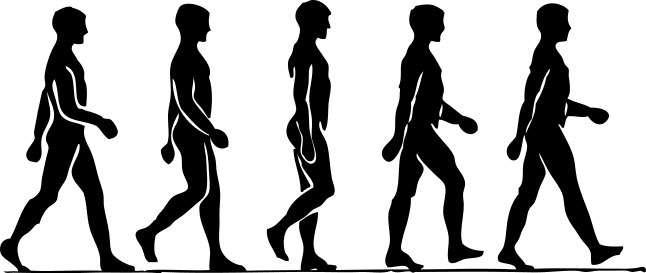
\includegraphics[width=0.90\columnwidth]{figures/human_locomotion.png}
\end{center}
\caption{Locomotion: \textit{``The movement of an organism from one place to another, oftenby the action of appendages such as flagella, limbs, or wings. Insome animals, such as fish, locomotion results from a wavelikeseries of muscle contractions.}'' -- The American Heritage Science Dictionary. Image source: wpclipart.com.}
\end{figure}

Our source code is available at \url{https://github.com/jeffton/Pervasive-Assignment-3}.

\section{Background}

Sensor data is often relevant in ubicomp applications as it deals with implicit input. Context-aware applications can use sensors to detect ongoing activities and automatically adjust their behavior to fit the current situation. Sensors typically provide large amounts of data, sometimes with inaccuracies or noise, and usually with a level of indirection towards what the application actually needs to know. As an example, motion detectors and microphones can be used to try to determine whether or not someone is in a room, even if this true-or-false-statement is not directly measured by the sensors. Data processing techniques enter the picture as a means to make sense of such sensor data.
The data analysis in this assignment is a case of supervised learning: classification of training data lets us predict the class of new data.

\section{The system}

The system, consisting of the Android app and a Google App Engine (GAE) service, is composed of three packages, \lstinline[mathescape]{app}, \lstinline[mathescape]{shared}, and \lstinline[mathescape]{service}, all located in the \lstinline[mathescape]{dk.itu.spct.locomotion} namespace. The \lstinline[mathescape]{shared} package holds the two classes \lstinline[mathescape]{LocomotionData} and \lstinline[mathescape]{DataPoint}, which are used to store and serialize the recorded motion data in. The \lstinline[mathescape]{LocomotionData} class is used to represent a single recording, and the \lstinline[mathescape]{DataPoint} class is used to represent a single event in a recording. See figure \ref{fig:classDiagram} for details.

\begin{figure}[th]
\begin{center}
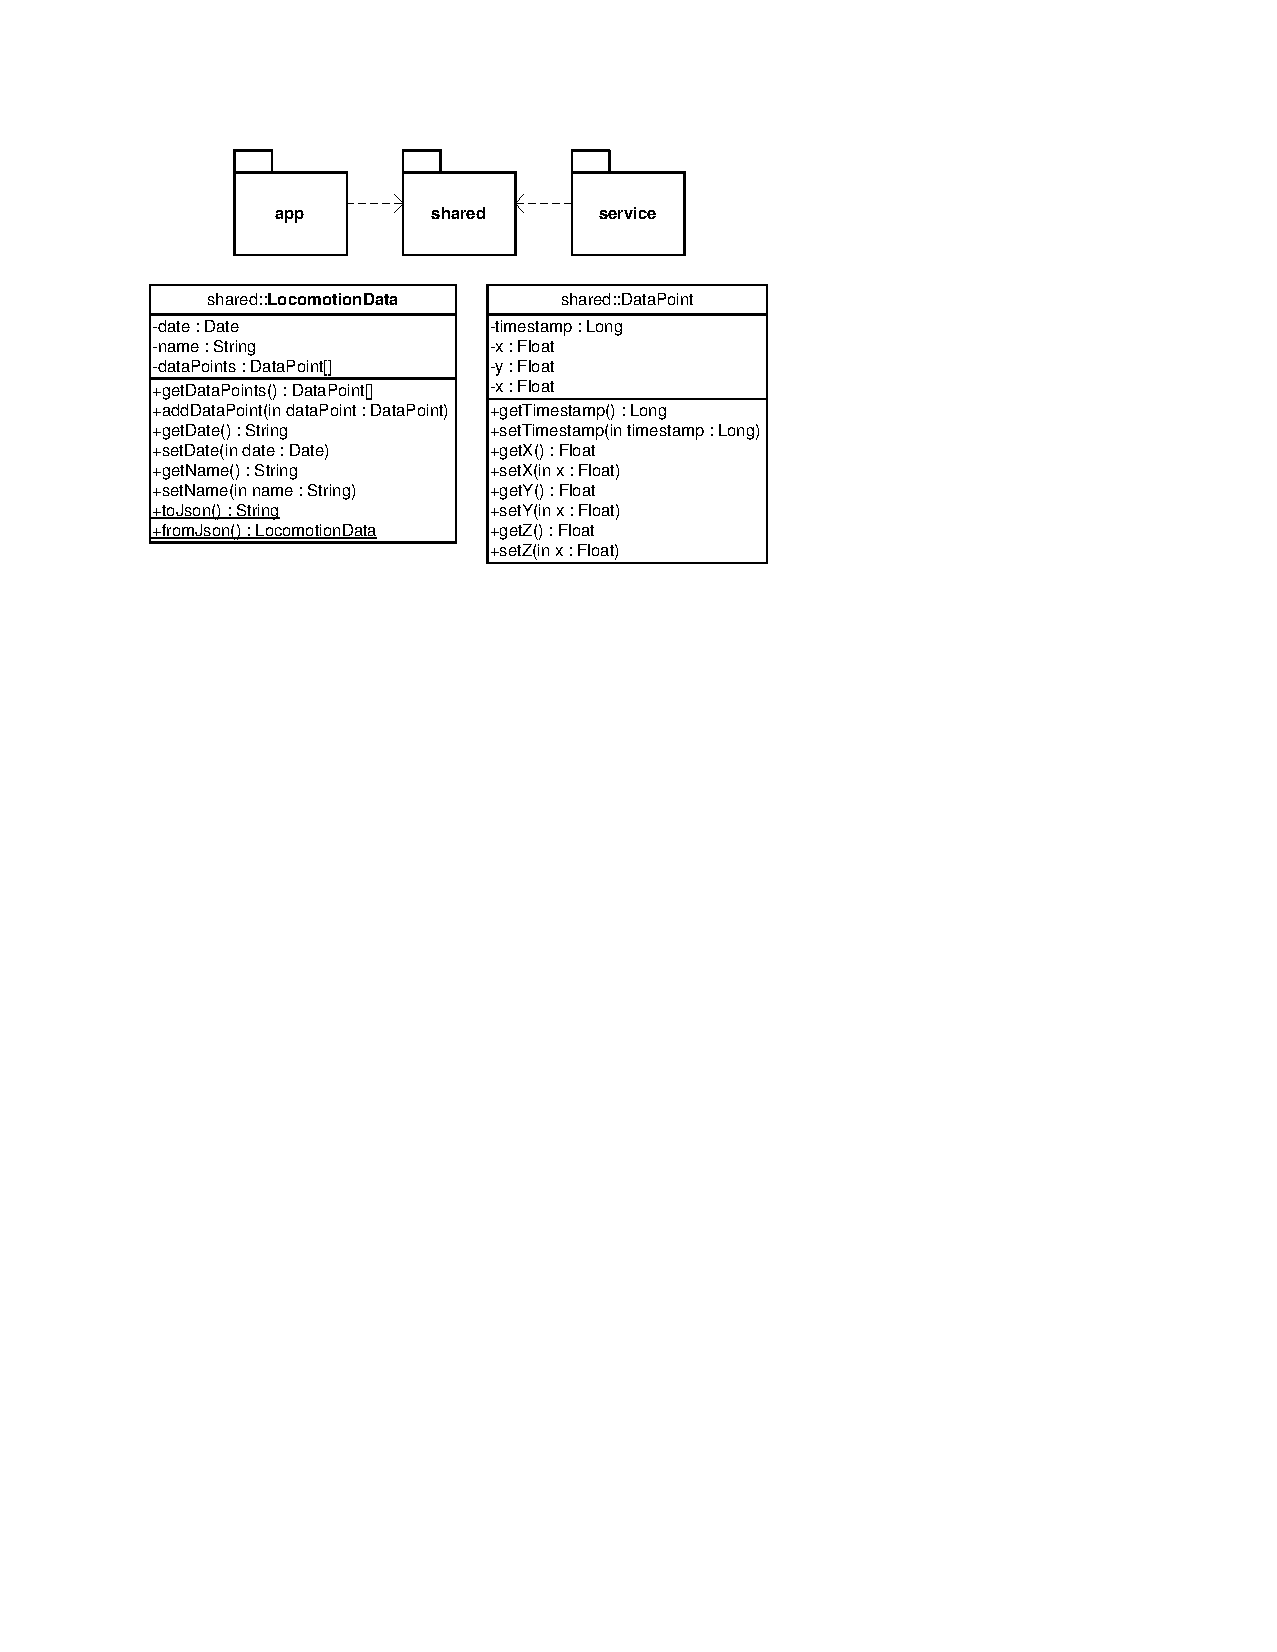
\includegraphics[width=0.90\columnwidth]{figures/class-diagram.pdf}
\end{center}
\caption{System packaged diagram and class diagram for the shared classes.}
\label{fig:classDiagram}
\end{figure}

\subsection{The Android App}

The Android app consists of a single activity, \lstinline[mathescape]{RecordingA$\\$ctivity}, that allows the user to record and upload a set of accelerometer data. The recording itself is handled by our \lstinline[mathescape]{AccelerometerRecorder} class which uses the accelerometer of the Android phone via \lstinline[mathescape]{SensorManager.getDefaultSensor(Sensor.TYPE_ACCELEROMET$\\$ER)}.
After pressing the record button, the app waits a couple of seconds before actually starting the recording to allow the user to get ready. The phone vibrates before and after recording to inform the user.

Once the recording is complete, the user is prompted to name and save the recording. If the prompt is confirmed, the recording, now including the provided name and the current time, is serialized to JSON using google-gson\footnote{\url{http://code.google.com/p/google-gson/}} and sent to the service using our \lstinline[mathescape]{DataUploader} class.

\subsection{Service on Google App Engine}

The service consists of two servlets, one that handles upload of locomotion data, i.e. \lstinline[mathescape]{UploadServlet}, and one that serves the data back again to the user, i.e. \lstinline[mathescape]{GetDataSer$\\$vlet}. The service also has a simple HTML-based front-end\footnote{Available at \url{http://locomotion-at-itu.appspot.com/}.} component that enables users to perform test uploads and download already uploaded locomotion data. Upon upload, the raw locomotion data stored in \lstinline[mathescape]{LocomotionData} object is converted to a CSV file and then stored in GAE’s Blobstore. We use the Blobstore since it allows us to serve the saved CSV files directly with a simple API call, keeping the code very simple.

\section{Capturing Training Data}

We captured data for three different activities: walking, sitting, and ascending stairs. Two people, each using their own phone, performed each activity five times. This gave us a total of 30 recordings, each with a duration of 10 seconds with 20 samples per second. The phone was placed in a pants pocket while recording.

Table \ref{sampleData} shows a snippet of one recording. The timestamps are in nanoseconds and are relative to the beginning of the recording. Note how some preprocessing is already taken care of while recording: besides saving relative timestamps, the app makes it easy to carry out the recorded activities during the entire recording. This removes the need to cut the beginning and end of the recordings afterwards.

\begin{table}[]
\small
\def\arraystretch{1.5}
  \begin{tabular}{rS[table-format=3.8]S[table-format=3.7]S[table-format=3.9]}
  \toprule
  \multicolumn{1}{c}{\textbf{Timestamp}} & \multicolumn{1}{c}{X} & \multicolumn{1}{c}{Y} & \multicolumn{1}{c}{Z} \\
  \midrule
  0         & -7.434141   &  -6.09293   & -5.364844 \\
  49377444  & -2.1459377  & -17.665665  & -0.45984375 \\
  98907476  & -2.0309765  & -10.844649  & -2.2608986 \\
  149383550 & -2.567461   & -13.756992  & -0.728086 \\
  199340826 & -1.6094532  & -11.917618  & -0.038320314 \\
  249328617 & -1.7627344  & -10.308165  & -0.0 \\
  299774174 & -2.2608986  &  -9.081915  & -0.45984375 \\
  349426272 &  0.15328126 &  -6.5144534 &  0.5364844 \\
  399230958 &  0.11496094 &  -8.047266  &  0.4981641 \\
  449218750 & -1.9926564  &  -8.277188  &  0.38320315 \\
  502990721 & -2.7973828  & -11.726016  & -0.4981641 \\
  549591062 & -2.6441016  & -12.032578  & -1.0346485 \\
  599182127 &  1.22625    & -15.174845  & -2.3375392 \\
  653045652 & -3.8703518  & -14.944922  & -0.8047266 \\
  699218748 &  0.45984375 & -13.48875   & -1.8010547 \\
  749206540 & -1.1112891  & -12.032578  & -2.912344 \\
  799560544 & -0.07664063 & -7.702383   & -1.4944923 \\
  849243162 & -3.908672   & -4.8283596  & -0.45984375 \\
  899597166 & -0.6514453  & -4.3301954  & -1.0729688 \\
  949584959 & -0.8430469  & -3.3338673  & -2.2225783 \\
  \bottomrule
  \end{tabular}
  \caption{Sample locomotion data. This is the first second of a recording where a person is ascending stairs.}
  \label{sampleData}
\end{table}

\section{Data Processing with Weka}

In order to use our data in Weka we needed to preprocess it into a suitable format. The first part was already done in our Android application where we changed the timestamps of the data points to be relative to the beginning of the recording rather than absolute timestamps. The next preprocessing we performed was to manually label the recordings as walking, sitting or ascending stairs. As our application starts after 5 seconds and runs in 10 seconds, we have decided not to remove the first and last couple of recordings.

If we make a 10 fold cross validation with our training set, we get 76\% correctly classified instances and the confusion matrix in table \ref{secondConfusionMatrix}.

\begin{table}[!h]
\centering
\def\arraystretch{2}
\begin{tabular}{p{1cm}p{1cm}p{1cm}l}
\toprule
\textbf{a} & \textbf{b} & \textbf{c} & \textbf{Classified as} \\
\midrule
1018 & 2 & 897 & a = stairs \\
1 & 1963 & 5 & b = sit \\
474 & 9 & 1431 & c = walk \\
\bottomrule
\end{tabular}
\caption{Confusion matrix for 10 fold cross validation.}
\label{secondConfusionMatrix}
\end{table}

After making the 10 recordings of each activity, we have tried to classify another recording in Weka. When using a Bayes network algorithm, we get 67,9\% correctly classified instances with the confusion matrix in table \ref{firstConfusionMatrix}

\begin{table}[!h]
\centering
\def\arraystretch{2}
\begin{tabular}{p{1cm}p{1cm}p{1cm}l}
\toprule
\textbf{a} & \textbf{b} & \textbf{c} & \textbf{Classified as} \\
\midrule
199 & 0 & 1 & a = stairs \\
0 & 199 & 0 & b = sit \\
190 & 0 & 7 & c = walk \\
\bottomrule
\end{tabular}
\caption{Confusion matrix using the Bayes network algorithm.}
\label{firstConfusionMatrix}
\end{table}

Here we are able to see that the algorithm categorizes all the movements as walking on stairs.
\newline
\newline
\section{Discussion}

In our training we have used two different kinds of phones and two people have been walking with each. This gives some better value to the data, as people have different ways of moving, and the phones can also have different values for the same operation. In order to gain even better results we also have to be aware that values can change if the phone is placed upside down, or with the screen towards the body or away from the body. So in order to gain a higher percentage of correctly classified instances, we need to get training data from more phones, persons and make sure that the phones is in different positions. But we will never get a 100% classification, as there will always be differences in the data.

\section{Conclusion}

In this assignment, we have recorded time series of accelerometer data from an Android phone while performing various activities.

By classifying the recordings and using them as a training set in Weka, we have been able to determine the activities performed in new recordings with an accuracy of 67.9\% -- our main problem being that walking was incorrectly classified as the rather similar activity of ascending stairs.


\end{document}
